\documentclass[10pt]{IEEEtran}
\usepackage{graphicx}
\usepackage{amsmath}
\usepackage{hyperref}
\usepackage{listings}
\usepackage{xcolor}
\usepackage{booktabs} 
\usepackage{textcomp}  % For \textrightarrow
\usepackage{amssymb}   % For \leq and \geq
\usepackage{tabularx}  % For better table control
\usepackage{booktabs}  % For professional tables
\usepackage{tikz}
\usepackage{pgfplots}


% Define Rust language for listings
\lstdefinelanguage{Rust}{
    keywords={pub, enum, struct, impl, fn, let, mut, Arc, Mutex, Vec, Option, String, u64, u16, u8, i32, Result, Ok, Err, Self, self, true, false, None, Some},
    sensitive=true,
    comment=[l]{//},
    morecomment=[s]{/*}{*/},
    string=[b]",
    stringstyle=\color{red},
    keywordstyle=\color{blue},
    commentstyle=\color{green!60!black},
    basicstyle=\small\ttfamily,
    breaklines=true,
    frame=single,
    numbers=none,
    showstringspaces=false,
    columns=flexible,
    keepspaces=true,
    xleftmargin=2em,
    xrightmargin=2em
}

% Add lstlisting style definitions
\lstset{
    basicstyle=\small\ttfamily,
    breaklines=true,
    frame=single,
    numbers=none,
    showstringspaces=false,
    keywordstyle=\color{blue},
    stringstyle=\color{red},
    commentstyle=\color{green!60!black},
    morekeywords={pub, enum, struct, impl, fn, let, mut, Arc, Mutex, Vec, Option, String, u64, u16, u8, i32, Result, Ok, Err},
    columns=flexible,
    keepspaces=true,
    xleftmargin=2em,
    xrightmargin=2em
}

\title{RepliCode: Deterministic Replication for WebAssembly Runtimes via Ordered I/O}

\author{
    \IEEEauthorblockN{Ricardo Perelló Mas \\}
    \IEEEauthorblockA{
        Distributed Computing Lab, EPFL \\
        ricardo.perellomas@epfl.ch \\
        Spring 2025
    }
}

\date{\today}

\begin{document}

\maketitle

\begin{abstract}
RepliCode introduces a deterministic WebAssembly runtime designed for replicated systems. It enables consistent execution across distributed nodes by enforcing a shared order of external I/O operations through a deterministic consensus mechanism. At the heart of RepliCode is a NAT-inspired network abstraction layer that orchestrates connection lifecycles, port mappings, and I/O buffering in a way that is replayable and consistent across all replicas. This report presents the design, implementation, and evaluation of RepliCode, showing that it supports elastic scaling, deterministic synchronization of new replicas, and practical performance with minimal overhead.
\end{abstract}

\section{Introduction}

\subsection{Motivation}
Modern cloud and distributed systems increasingly serve as the backbone of critical infrastructure, including financial platforms, health systems, and national security services. These systems often replicate services across nodes to ensure availability and resilience. However, replication alone is insufficient if nodes exhibit divergent behavior due to non-determinism. For example, in replicated key-value stores, slight differences in execution order or timing can lead to inconsistency and state divergence. In high-stakes scenarios such as digital voting or secure database replication, even minor inconsistencies represent security vulnerabilities.

Ensuring bit-for-bit identical behavior across replicas is thus essential. Unfortunately, most existing solutions either rely on restrictive programming models, avoid I/O entirely, or require heavyweight checkpointing and replay. None of these solutions scale well in environments with dynamic nodes, real-time interactions, or adversarial threat models. RepliCode represents an exploratory step toward addressing this gap, investigating the feasibility of a deterministic execution platform that fully supports I/O and networking while guaranteeing consistent outputs across replicas. While not yet optimized for production deployment, this proof-of-concept demonstrates the potential for practical deterministic replication in real-world distributed systems.

\subsection{Contributions}
RepliCode contributes a new execution model and system architecture that provides determinism without sacrificing interactivity or elasticity. Its key contributions are:

\begin{itemize}
    \item \textbf{Deterministic Network Operation Layer:} A NAT-inspired component that handles port assignment, connection routing, and buffering in a globally consistent manner.
    \item \textbf{Per-Process Isolation and Port Management:} Runtime-level separation of port spaces, with deterministic assignment and state tracking.
    \item \textbf{Runtime Synchronization Mechanism:} A replay-based system that allows new runtime replicas to deterministically reconstruct global state without halting execution.
    \item \textbf{Comprehensive Test Suite:} A collection of client-server applications that validate and demonstrate the system's deterministic behavior, synchronization capabilities, and networking abstractions.
\end{itemize}

\section{Background}

\subsection{Determinism in Distributed Systems}
Determinism ensures that a system produces the same output given the same input \cite{deterministic2010}. In replicated systems, determinism is a prerequisite for correctness: if replicas diverge due to timing differences or nondeterministic behaviors (e.g., thread scheduling, I/O race conditions), the system can fail. Traditional replicated state machines (RSMs) solve this by requiring that all replicas execute operations in the same global order \cite{deterministic2010}.

However, RSMs often avoid or restrict external I/O to maintain determinism \cite{deterministic2009}. They rely on primary-backup models, custom languages, or disable networking entirely. This makes them impractical for general-purpose distributed applications that interact with the outside world.

\subsection{WebAssembly and WASI}
WebAssembly (WASM) is a portable binary instruction format designed for safe, sandboxed execution \cite{wasm2017}. WASI extends WASM with a set of system interface APIs, enabling I/O, networking, and file access \cite{wasi2023}. While WASM provides portability and isolation, it does not address nondeterminism: system calls, thread scheduling, and network interactions can behave differently across executions \cite{wasm2020}.

RepliCode builds on WASM and WASI by intercepting and managing these external effects through a deterministic runtime. This allows real-world WASM applications to be replicated with full consistency, even across dynamic deployments.

\subsection{Deterministic NAT Abstractions}
Network Address Translation (NAT) abstracts internal and external port spaces, typically for isolation or routing purposes. RepliCode extends this idea into a deterministic coordination tool: instead of simply mapping ports, it mediates all connection lifecycles, buffers, and I/O to ensure replayability \cite{deterministic2009}. This guarantees that all runtimes observe the same connection events and message streams in the same order.

\subsection{Runtime Synchronization}
One challenge of distributed systems is bringing new nodes into sync without halting the system \cite{elastic2016}. While RepliCode employs a log-based synchronization mechanism, a complete system could optionally integrate periodic snapshots, typically by dumping the WASM memory of user processes. This would be particularly useful for long-running services where disk capacity for logs is finite. RepliCode avoids halting execution by replaying the entire history of incoming batches to new runtimes. Since all effects are deterministic and ordered, this replay guarantees state equivalence \cite{consistency2015}.

The ability to join mid-execution and become immediately consistent is key to RepliCode's elastic scaling model and fault recovery strategy.

\section{System Design}

The RepliCode architecture consists of two core components: a centralized \textbf{consensus server} and multiple distributed \textbf{replicated runtimes}. The consensus server coordinates external I/O operations and enforces deterministic execution by maintaining and broadcasting ordered sequences of operations known as \emph{batches}. Critically, \textbf{all communication} between the consensus server and runtimes occurs exclusively through these batches, ensuring strict determinism and consistency across the system.

A \textbf{batch} is an ordered set of high-level \emph{commands}, representing either user inputs or external system events. Each batch is finalized by appending a logical clock tick, creating a global timeline shared by all runtimes. The global clock ensures that all runtimes process events in the same order, even if they have different processing speeds or resource constraints. Batches are generated at configurable fixed intervals, ensuring consistent timing across all runtime instances.

\subsection{Consensus Server}

The consensus server acts as the central authority and performs four primary roles:

\begin{itemize}
\item \textbf{NAT Module:} Provides deterministic network management, handling port mappings, message routing, and maintaining network state consistency.
\item \textbf{Runtime Manager:} Manages runtime connections, session states, and runtime availability. If a runtime disconnects, it is immediately removed from the distribution list to maintain consistency.
\item \textbf{HTTP Server:} Publishes NAT mappings publicly, allowing external clients to discover the correct ports for interacting with services running inside runtimes.
\item \textbf{Command Interface:} Accepts user commands via a command-line interface (CLI), buffering them until the batch timer triggers batch creation.
\end{itemize}

It is important to note that while we refer to this component as a "consensus server," it is in reality a simplified abstraction of a true consensus mechanism. The server acts as a centralized authority that enforces deterministic ordering of operations, rather than implementing a full Byzantine fault-tolerant consensus protocol. This design choice was made to focus on the core challenges of deterministic execution and network operation ordering, while acknowledging that a production system would require a more robust consensus mechanism to handle Byzantine failures and ensure true distributed consensus.

Upon each timer expiration, the consensus server aggregates buffered user commands and intercepted I/O operations, appends a logical timestamp, and broadcasts this batch to all connected runtimes. All batches are persistently logged.

\subsection{Runtime Design}

Each runtime is sandboxed and executes batches deterministically. Runtimes consist of the following key components:

\begin{itemize}
\item \textbf{Consensus Input Buffer:} Stores incoming batches from the consensus server until they are ready for processing.
\item \textbf{Deterministic Scheduler:} Controls execution of processes according to batch order and local runtime state, ensuring deterministic outcomes.
\item \textbf{I/O Interceptor:} Captures all system calls related to external operations, redirecting them through consensus-managed pathways.
\item \textbf{Outgoing Buffer:} Collects intercepted I/O calls, bundling them into an outgoing batch sent back to the consensus server before processing new incoming batches.
\end{itemize}

Each runtime maintains detailed per-process metadata—including execution state, blocking conditions, and a local NAT table—to facilitate deterministic scheduling decisions. Importantly, each process maintains its own isolated NAT state, distinct from the public NAT mappings maintained by the consensus server. 

Since runtimes deterministically execute identical incoming batches, their outgoing batches are inherently identical. The consensus server accepts the first received outgoing batch from any runtime, discarding duplicates. This design choice simplifies the implementation while maintaining determinism, though it does not provide Byzantine fault tolerance.

The RepliCode architecture abstracts network interactions completely. Both clients and internal processes perceive their interactions as direct socket communication, while all underlying coordination—such as batching and NAT mappings—is hidden, preserving conventional networking semantics.

\subsection{Synchronization Mechanism}
When a new runtime instance joins the system, it must be brought into a fully consistent state with respect to existing replicas. RepliCode achieves this through a dedicated synchronization mechanism implemented by the consensus server's runtime manager.

Upon connection, the runtime manager assigns the new runtime a unique identifier and retrieves all previously issued incoming batches from the persistent batch log. These batches represent the entire historical sequence of system events. The manager sequentially transmits these batches to the new runtime in the exact order they were originally generated. Because all commands are deterministic and batches encode a complete history, the joining runtime reconstructs its state precisely from the initial execution state to the present.

Critically, determinism at the runtime level is guaranteed by stripping inherent non-determinism from external I/O at the consensus level, which ensures that all instructions are processed in a consistent order within batches. Subsequently, each runtime, using carefully designed system call implementations and a custom scheduler, ensures that identical inputs and state produce exactly the same result. This combined approach results in total state determinism, allowing runtimes to synchronize seamlessly and remain consistently synchronized thereafter.

This mechanism guarantees that newly connected runtimes behave identically to existing ones and can participate in future batch processing immediately after synchronization—without disrupting consensus or requiring any global pause. This elasticity is a cornerstone of RepliCode's design, enabling dynamic scaling and fault recovery with minimal operational overhead.

\subsection{Execution Flow}

The following steps illustrate the high-level execution flow in RepliCode:

\begin{enumerate}
\item The consensus server initializes and begins accepting runtime connections.
\item New runtimes connect and are synchronized by receiving and replaying all historical incoming batches.
\item A user initiates a server process through the consensus server's command interface.
\item The consensus server adds the init command to the next batch.
\item Runtimes execute commands in the precise order dictated by incoming batches.
\item When a runtime process issues an external I/O call, it is intercepted and buffered.
\item Buffered I/O calls are sent back as an outgoing batch to the consensus server before the next incoming batch is processed.
\item The consensus server processes these outgoing batches, updating NAT state, and prepares any resulting events (e.g., network responses) for inclusion in the subsequent batch.
\item Updated batches are sent to runtimes, continuing the deterministic execution loop.
\end{enumerate}


\subsection{NAT Layer Operation}

The NAT module provides deterministic management of network interactions. It operates through a structured mapping mechanism, maintaining consistent port assignments and connection states across all runtimes. The key components and responsibilities of the NAT module include:

\begin{itemize}
\item \textbf{Port Allocation and Mapping:} The NAT assigns public ports deterministically to internal process sockets upon request, maintaining consistent mappings across all replicas. Each process-socket pair receives a unique public port to avoid conflicts.
\item \textbf{Connection Management:} NAT tracks connections initiated by runtimes, maintaining mappings between internal and consensus-level ports. It manages connection lifecycles explicitly, handling establishment, data forwarding, and termination deterministically.
\item \textbf{Buffering and Forwarding:} Incoming data from external clients is buffered by NAT until requested by processes. NAT forwards data deterministically, ensuring all runtimes receive identical data streams at the same points in their execution.
\item \textbf{Non-blocking Operations and Waiting States:} Operations such as \texttt{accept} and \texttt{recv} may temporarily block if no data or connections are available. NAT manages these states explicitly, marking operations as waiting and resuming them once the relevant events occur.
\end{itemize}

This deterministic and structured approach ensures consistent network behavior across all runtime replicas, facilitating strong consistency.


\subsection{NAT Interaction Example}

The following example demonstrates deterministic NAT interactions, where an image server is running inside a runtime with process id = 2 and an external client is sending requests to the server, with diagrams illustrating the step-by-step communication:

\textbf{Step 1 (Connection Setup):}
\begin{enumerate}
\item Server process listens on internal port 7000.
\item Consensus server assigns public port 10000 mapped to \texttt{pid2:7000}.
\item Server blocks waiting for client connection.
\item Client queries consensus HTTP server, discovering public port 10000 for \texttt{pid2:7000}.
\item Client initiates connection to port 10000.
\item Consensus registers new connection, assigning internal port 8000 and public port 10001.
\item Connection setup completes successfully.
\end{enumerate}

\begin{figure}[h]
\centering
\includegraphics[width=0.9\linewidth]{consensus_diagram_1.pdf}
\caption{Step 1: Initial connection setup and port assignment.}
\label{fig:consensus-1}
\end{figure}

\textbf{Step 2 (Data Transfer):}
\begin{enumerate}
\item Client sends file \texttt{lake.jpg} to port 10001.
\item Server reads data from internal port 8000.
\item NAT forwards data deterministically.
\item Server closes the connection, and NAT cleans up mappings.
\end{enumerate}

\begin{figure}[h]
\centering
\includegraphics[width=0.9\linewidth]{consensus_diagram_2.pdf}
\caption{Step 2: Deterministic message routing and data transfer.}
\label{fig:consensus-2}
\end{figure}

\textbf{Step 3 (Handling Additional Connections):}
\begin{enumerate}
\item Server accepts new connection on internal listener port 7000.
\item Client connects via public port 10000.
\item NAT assigns new public port 10002.
\item Client sends request \texttt{"GET lake.jpg"} to port 10002.
\item NAT forwards request to internal port 8001.
\item Server responds, and NAT forwards the response back to the client.
\item Connection closes gracefully.
\end{enumerate}

\begin{figure}[h]
\centering
\includegraphics[width=0.9\linewidth]{consensus_diagram_3.pdf}
\caption{Step 3: Handling new connections and request/response flow.}
\label{fig:consensus-3}
\end{figure}

Figures \ref{fig:consensus-1}, \ref{fig:consensus-2}, and \ref{fig:consensus-3} visually represent each step of this deterministic interaction.


\section{Implementation Details}

This section details the implementation of RepliCode's consensus server, which orchestrates deterministic execution across distributed runtime instances. The server is implemented in Rust and consists of several key components that work together to ensure consistent state and operation ordering.

\subsection{Consensus Server Architecture}

The consensus server manages runtime connections and coordinates network operations through a deterministic NAT layer. The server's architecture consists of five main components:

\begin{itemize}
    \item \textbf{Controller:} Coordinates all server components and maintains the main command loop.
    \item \textbf{Runtime Manager:} Handles runtime connections and batch distribution.
    \item \textbf{NAT Layer:} Provides deterministic network operation ordering.
    \item \textbf{HTTP Server:} Exposes NAT mappings for external client discovery.
    \item \textbf{Batch System:} Manages command batching and clock synchronization.
\end{itemize}

\subsection{Controller}

The controller (\texttt{Controller}) serves as the central coordinator, initializing and managing all server components. Its key responsibilities include:

\begin{itemize}
    \item Starting and monitoring runtime connections
    \item Managing the batch sender thread
    \item Coordinating the runtime reader thread
    \item Overseeing the NAT checker thread
    \item Maintaining the HTTP server
    \item Processing user commands
\end{itemize}

The controller ensures that all components operate in a synchronized manner, with each component running in its own thread to maintain responsiveness and handle concurrent operations.

\subsection{Runtime Manager}

The runtime manager (\texttt{RuntimeManager}) handles all aspects of runtime connectivity and batch distribution. It maintains:

\begin{itemize}
    \item A map of connected runtimes with their unique identifiers
    \item Per-runtime connection state and last processed batch numbers
    \item Batch history for new runtime synchronization
\end{itemize}

When a new runtime connects, the manager:
\begin{enumerate}
    \item Assigns a unique runtime ID
    \item Retrieves historical batches from persistent storage
    \item Transmits these batches to synchronize the new runtime
    \item Adds the runtime to the active connection pool
\end{enumerate}

The manager also implements batch broadcasting, ensuring that all runtimes receive the same sequence of operations in the same order. This is achieved through a deterministic batch numbering system and careful tracking of each runtime's last processed batch.

\subsection{NAT Layer}

The NAT layer (\texttt{NatTable}) provides deterministic network operation ordering through a sophisticated port mapping and connection management system. Key features include:

\begin{itemize}
    \item \textbf{Port Mapping:} Maintains bidirectional mappings between process ports and consensus-level ports
    \item \textbf{Connection Tracking:} Manages active connections and their states
    \item \textbf{Listener Management:} Handles server sockets and pending connections
    \item \textbf{Buffering:} Implements deterministic message buffering for reliable delivery
\end{itemize}

The NAT layer supports several network operations:
\begin{lstlisting}[language=Rust]
enum NetworkOperation {
    Connect { 
        dest_addr: String,
        dest_port: u16,
        src_port: u16
    },
    Send { 
        src_port: u16,
        data: Vec<u8>
    },
    Close { 
        src_port: u16
    },
    Listen { 
        src_port: u16
    },
    Accept { 
        src_port: u16,
        new_port: u16
    },
    Recv { 
        src_port: u16
    }
}
\end{lstlisting}

Each operation is processed deterministically, with the NAT layer maintaining consistent state across all runtime instances. The layer also implements waiting states for operations like \texttt{accept} and \texttt{recv}, ensuring that processes block appropriately when no data or connections are available.

\subsection{HTTP Server}

The HTTP server component provides a REST API for external clients to discover and interact with services running inside the runtimes. It exposes:

\begin{itemize}
    \item Process information and port mappings
    \item Active connection details
    \item Listener status and pending accepts
\end{itemize}

This information is crucial for external clients to locate the correct consensus-level ports for connecting to services running inside the runtimes.

\subsection{Batch System}

The batch system implements a deterministic command batching mechanism. Each batch consists of:

\begin{lstlisting}[language=Rust]
struct Batch {
    number: u64,
    direction: BatchDirection,
    data: Vec<u8>
}
\end{lstlisting}

Batches can be either \texttt{Incoming} (from consensus to runtime) or \texttt{Outgoing} (from runtime to consensus). The system:

\begin{itemize}
    \item Aggregates commands and network operations into batches
    \item Appends logical clock ticks to maintain global timing
    \item Broadcasts batches to all connected runtimes
    \item Persists batch history for runtime synchronization
\end{itemize}

The batch sender thread creates new batches at configurable fixed intervals, ensuring consistent timing across all runtime instances. Each batch includes a clock record to maintain synchronization.

\subsection{Command Processing}

The consensus server supports several high-level commands:

\begin{lstlisting}[language=Rust]
enum Command {
    Clock(u64),
    Init { 
        wasm_bytes: Vec<u8>, 
        dir_path: Option<String>, 
        args: Vec<String> 
    },
    FDMsg(u64, Vec<u8>),
    NetworkIn(u64, u16, Vec<u8>),
    NetworkOut(u64, NetworkOperation)
}
\end{lstlisting}

These commands are processed through a command-line interface, with each command being:
\begin{enumerate}
    \item Parsed and validated
    \item Converted to a record
    \item Added to the shared buffer
    \item Included in the next batch
\end{enumerate}

The command processing system ensures that all operations are properly ordered and synchronized across runtime instances, maintaining determinism throughout the system.

\subsection{Runtime Implementation}

The runtime component is responsible for executing WebAssembly processes deterministically while maintaining synchronization with the consensus server. It consists of several key components that work together to ensure consistent execution across all instances:

\begin{itemize}
    \item \textbf{Process Management:} Handles process creation, isolation, and state tracking.
    \item \textbf{Deterministic Scheduler:} Controls execution order and process scheduling.
    \item \textbf{Network Operations:} Implements deterministic network system calls.
    \item \textbf{Consensus Input Processing:} Manages batch processing and state updates.
    \item \textbf{Process Isolation:} Ensures sandboxed execution and resource limits.
\end{itemize}

A key aspect of the runtime's determinism is its use of a custom global clock implementation rather than the system's real-time clock. This clock, implemented as an atomic counter, ensures that all runtime instances maintain synchronized timing without relying on potentially divergent system timestamps.

\subsection{Process Management}

The runtime implements a sophisticated process management system through the \texttt{Process} and \texttt{ProcessData} structures:

\begin{lstlisting}[language=Rust]
pub struct Process {
    pub id: u64,
    pub thread: thread::JoinHandle<()>,
    pub data: ProcessData
}
\end{lstlisting}
\begin{lstlisting}[language=Rust]
pub struct ProcessData {
    pub fd_table: Arc<Mutex<FDTable>>,    
    pub state: Arc<Mutex<ProcessState>>,  
    pub block_reason: Arc<Mutex<Option<BlockReason>>>,
    pub next_port: Arc<Mutex<u16>>,
    pub network_queue: Arc<Mutex<Vec<OutgoingNetworkMessage>>>,
    pub nat_table: Arc<Mutex<NatTable>> 
}
\end{lstlisting}

Each process maintains its own isolated state, including:
\begin{itemize}
    \item Execution state (Ready, Running, Blocked, Finished)
    \item Blocking conditions for I/O operations
    \item File descriptor table for I/O management
    \item Network queue for outgoing messages
    \item Local NAT table for network state
\end{itemize}

\subsection{Deterministic Scheduler}

The runtime implements a dynamic scheduler that ensures deterministic execution of processes. The scheduler maintains two queues:

\begin{itemize}
    \item \textbf{Ready Queue:} Contains processes ready for execution
    \item \textbf{Blocked Queue:} Contains processes waiting for I/O or other events
\end{itemize}

The scheduler operates in a loop that:
\begin{enumerate}
    \item Executes all ready processes until they block or yield
    \item Processes consensus input to update process states
    \item Attempts to unblock processes based on their block reasons
    \item Maintains synchronization with the global clock
\end{enumerate}

Key features of the scheduler include:
\begin{itemize}
    \item Deterministic process ordering
    \item Non-blocking I/O operations
    \item Batch-based execution
    \item Global clock synchronization
\end{itemize}

\subsection{Network Operations}

The runtime implements a deterministic network layer through WASI-compatible system calls. Key operations include:

\begin{lstlisting}[language=Rust]
pub fn wasi_sock_open(...) -> i32
pub fn wasi_sock_connect(...) -> i32
pub fn wasi_sock_listen(...) -> i32
pub fn wasi_sock_accept(...) -> i32
pub fn wasi_sock_send(...) -> i32
pub fn wasi_sock_recv(...) -> i32
pub fn wasi_sock_close(...) -> i32
\end{lstlisting}

Each network operation:
\begin{enumerate}
    \item Validates parameters and state
    \item Queues the operation in the process's network queue
    \item Blocks the process until consensus processes the operation
    \item Updates local NAT state based on consensus response
\end{enumerate}

The network layer ensures determinism by:
\begin{itemize}
    \item Maintaining consistent port assignments
    \item Buffering messages until consensus confirmation
    \item Synchronizing connection states across runtimes
    \item Implementing deterministic waiting states
\end{itemize}
\subsection{Consensus Input Processing}

The runtime processes consensus input through a structured batch system:

\begin{lstlisting}[language=Rust]
pub fn process_consensus_pipe<R: Read + Write>(
    reader: &mut BufReader<R>,
    processes: &mut Vec<Process>,
    outgoing_messages: Vec<OutgoingNetworkMessage>
) -> Result<bool>
\end{lstlisting}

The input processor handles several types of commands:
\begin{itemize}
    \item \textbf{Clock Updates:} Synchronizes the global clock
    \item \textbf{FD Updates:} Manages file descriptor operations
    \item \textbf{Init Commands:} Creates new processes
    \item \textbf{Network Operations:} Processes network messages
    \item \textbf{Message Commands:} Handles inter-process communication
\end{itemize}

Each command is processed deterministically, with the system:
\begin{enumerate}
    \item Validating command parameters
    \item Updating process state
    \item Managing I/O operations
    \item Maintaining synchronization
\end{enumerate}

\subsection{Process Isolation}

The runtime ensures process isolation through several mechanisms \cite{replicode2025}:

\begin{itemize}
    \item \textbf{Sandboxed Execution:} Each process runs in its own WebAssembly instance
    \item \textbf{Resource Limits:} Processes have restricted disk and memory usage
    \item \textbf{Port Isolation:} Each process has its own port space
    \item \textbf{File System Isolation:} Processes have isolated file system access
\end{itemize}

Process creation involves:
\begin{enumerate}
    \item Allocating a unique process ID
    \item Creating a sandbox directory
    \item Initializing process state and resources
    \item Setting up the WebAssembly environment
    \item Registering system calls
\end{enumerate}

This isolation ensures that processes cannot interfere with each other while maintaining deterministic execution across all runtime instances \cite{replicode2025}.

\section{Evaluation}

\subsection{Setup}
\textbf{Hardware:} All experiments were conducted on identical machines with M4 PRO CPUs, 48 GB of RAM, and SSD storage, connected via a local area network. \\
\textbf{Software:} Each runtime was compiled using Rust (debug profile) and executed on macOS. We used debug mode to facilitate detailed debugging and logging during this development phase, though future performance-oriented evaluations should use Rust's optimized release mode. To demonstrate the system's capabilities, we implemented a simple TCP-based image server that handles file transfers through the NAT layer to external clients.

\subsection{Experiment 1: Network Overhead}
\textbf{Question:} What is the overhead introduced by the deterministic NAT layer in terms of bytes and latency? \\

\textbf{Method:} We compared file transfers between a direct client-server setup and one using the NAT layer. Transfers used 4 KB batching, where each batch carried up to 4096 bytes of payload plus a fixed 27-byte metadata header. \\

\textbf{Results:} The NAT layer consistently added 27 bytes of metadata per batch. For a small 3.6 KB file that fit entirely within a single partially filled batch (3686 bytes of payload), the total overhead was 27 bytes, or approximately 0.73\%. For a larger 2 MB file sent in 512 full batches of 4096 bytes each, the total metadata overhead amounted to 3629 bytes, or about 0.17\%. The NAT layer also introduced an additional 50 microseconds of latency per batch, in addition to the batch interval. \\

\textbf{Observations:}
\begin{itemize}
\item Overhead remained fixed at 27 bytes per batch
\item Relative overhead decreased as file size increased
\item Throughput was highly affected by both the batch interval and the batch size, with shorter intervals and larger batches yielding significantly better performance
\end{itemize}
\textbf{Deductions:}
\begin{itemize}
    \item Larger batches amortize the metadata cost more effectively
    \item The NAT layer achieves deterministic behavior with negligible overhead
\end{itemize}

\textbf{Conclusion:} The NAT layer introduces a small and predictable per-batch overhead. Its low impact on throughput and latency confirms its practicality for real-world deterministic systems.

\begin{figure}[h]
\centering
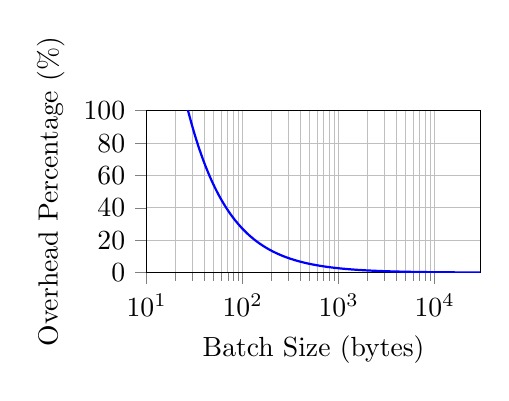
\begin{tikzpicture}
\begin{semilogxaxis}[
    xlabel={Batch Size (bytes)},
    ylabel={Overhead Percentage (\%)},
    xmin=10, xmax=30000,
    ymin=0, ymax=100,
    grid=both,
    legend style={at={(0.95,0.95)},anchor=north east},
    width=0.48\textwidth,
    height=0.3\textwidth,
    tick align=outside,
    tick pos=left
]
\addplot[blue, thick, domain=10:30000, samples=300] {27 / x * 100};

\end{semilogxaxis}
\end{tikzpicture}
\caption{Metadata overhead percentage as a function of batch size. The curve shows the overhead of 27 bytes per batch as a function of batch size.}
\label{fig:overhead}
\end{figure}\subsection{Experiment 2: Consistent File Transfers}
\textbf{Question:} Does the NAT layer ensure consistent operation ordering and data delivery across all runtime instances? \\
\textbf{Method:} Three runtime servers were launched. Clients performed SEND and GET operations for small, medium, and large files via the NAT. \\
\textbf{Observations:}
\begin{itemize}
    \item All runtime logs showed identical command sequences
    \item File contents and chunking were identical across all instances
    \item Timestamps across replicas were synchronized with minimal drift
\end{itemize}
\textbf{Deductions:}
\begin{itemize}
    \item The NAT layer enforces a consistent global operation order
    \item Data integrity is preserved even for large files
\end{itemize}
\textbf{Conclusion:} The system guarantees strong consistency and deterministic behavior across replicated servers, even during high-volume transfers.

\subsection{Experiment 3: Concurrent Operations}
\textbf{Question:} Can the NAT layer maintain deterministic behavior when multiple clients perform overlapping operations? \\
\textbf{Method:} We launched two clients. One initiated a SEND for a file while the second attempted a GET for that same file during the upload. We tested both directions to verify that connection timing, not request type, determined execution order. \\
\textbf{Observations:}
\begin{itemize}
    \item The NAT layer accepted and fully processed the first connection before serving the second
    \item Regardless of direction, the second client always received the fully completed file
    \item Runtime logs were identical across all instances
\end{itemize}
\textbf{Deductions:}
\begin{itemize}
    \item Connection order (first-come, first-served) fully determines execution order
    \item The NAT's single-threaded design prevents races and ensures deterministic replay
\end{itemize}
\textbf{Conclusion:} What matters is who connects first. The NAT layer's queue-based model guarantees that concurrent requests are serialized consistently across all runtimes, preserving determinism even in overlapping scenarios.

\subsection{Experiment 4: Buffer Management and Delivery Consistency}
\textbf{Question:} How well does the NAT layer's buffering system maintain consistent delivery and avoid corruption under high-throughput stress conditions? \\
\textbf{Method:} We transferred large files (10MB) through the NAT layer while systematically varying the batching interval between sends to identify the lower bound for reliable operation. Each batch consisted of 4 KB, and we tested a wide range of intervals, from sub-millisecond values to durations exceeding 15 ms, monitoring runtime behavior and system stability across all instances. \\
\textbf{Observations:}
\begin{itemize}
    \item Receiving Path: The system reliably handled batch intervals as low as $<$1ms, with all runtime replicas receiving identical byte sequences in the correct order
    \item Sending Path: When the batching interval dropped below 15ms, data corruption occurred. The NAT layer forwarded malformed messages
    \item Corrupted packets caused the consensus layer to crash, due to misinterpreted length fields triggering integer overflows during memory allocation
    \item At $\geq$15ms intervals, no corruption was observed, and deterministic delivery was preserved across all runtimes
\end{itemize}
\textbf{Deductions:}
\begin{itemize}
    \item The receiving path is robust under aggressive flushing conditions
    \item The sending path is sensitive to short intervals; premature flushing can lead to incomplete message construction
    \item Despite the corruption, data was always delivered in the same order across all instances, preserving determinism
\end{itemize}
\textbf{Conclusion:} The NAT layer enforces consistent delivery order under stress. However, we identified a bug in the implementation where sending in 4 KB batches with intervals below 15 ms leads to critical corruption and system crashes. This issue, caused by premature buffer flushing leading to malformed messages, is a fixable implementation problem for future iterations.

\subsection{Experiment 5: Deterministic Port Assignment}
\textbf{Question:} Does the system assign ports deterministically across replicated runtimes, ensuring isolation between processes without conflicts? \\
\textbf{Method:} We launched two distinct WASM services—an image server and a key-value server—across multiple runtime instances. The consensus driver initialized both services and routed all network operations through the deterministic NAT layer. We monitored the logs and port mappings to verify:
\begin{itemize}
    \item Per-process isolation of port spaces
    \item Deterministic and consistent port assignment across replicas
    \item Absence of collisions or reassignments after process restart
\end{itemize}
\textbf{Observations:}
\begin{itemize}
    \item When a process creates a socket, the NAT layer assigns a unique public port (e.g., 10001, 10002, 10003) to that socket, maintaining a mapping between process:socket and consensus:port
    \item No two processes ever shared the same port number within the same runtime
    \item The JSON NAT state confirmed disjoint listeners and mappings per process
    \item After process termination and restart, port counters resumed without reuse or error
    \item Logs were byte-for-byte consistent across all runtime instances
\end{itemize}
\textbf{Deductions:}
\begin{itemize}
    \item Port isolation is achieved through the NAT layer's centralized port allocation; each process's sockets are mapped to unique public ports
    \item Identical counter behavior in each replica guarantees deterministic port assignment
    \item The system avoids complexity (e.g., global registries or locking) without sacrificing correctness
\end{itemize}
\textbf{Conclusion:} The NAT-based design ensures deterministic, conflict-free port assignment across replicated runtimes. While a more traditional bind-based approach could be implemented in future work, the current design provides a clean abstraction for port management while maintaining consistency guarantees. Each process's sockets are mapped to unique public ports by construction, and assignment order remains consistent without additional coordination.

\subsection{Experiment 6: Dynamic Scaling}
\textbf{Question:} How efficiently can new runtime instances synchronize with the system during execution? \\
\textbf{Method:} We launched runtimes A, B, and C at staggered intervals ($T_0 + 9$s, $T_0 + 30$s, and $T_0 + 56$s respectively) and recorded synchronization metrics. \\
\textbf{Results:} New runtimes synchronized quickly, with join latencies of 182 ms, 197 ms, and 211 ms respectively. Each runtime processed an increasing number of historical batches (6, 20, and 37) with a linear metadata cost of approximately 54 bytes per batch. No consensus stalls were observed during the process.

\textbf{Observations:}
\begin{itemize}
    \item Latency remained low despite 6–37 batches being streamed
    \item Metadata cost scaled linearly, confirming our model of 54 B per batch
    \item No disruption to ongoing broadcast or execution was observed
\end{itemize}
\textbf{Deductions:}
\begin{itemize}
    \item The linear scaling of metadata cost suggests that the synchronization mechanism remains efficient even with large historical states
    \item The consistent join latencies across different batch counts indicate that the system's performance is not significantly impacted by the amount of historical data
    \item The absence of consensus stalls demonstrates that the synchronization process is well-integrated with the ongoing system operation
\end{itemize}
\textbf{Conclusion:} Even in the presence of large historical state, synchronization latency remained well below a single batch interval (150 ms), and all new runtimes converged deterministically to the current system state. The system incurred zero consensus backlog, and no flush exceeded 90 $\mu$s.

\subsection{Experiment 7: State Consistency During Operation}
\textbf{Question:} Do mid-execution joins preserve system consistency during I/O activity? \\
\textbf{Method:} We ran a multi-runtime setup with live image uploads. New runtimes were connected mid-transfer, and we verified that all runtimes (old and new) processed I/O identically and maintained convergent internal state. \\
\textbf{Observations:}
\begin{itemize}
    \item All runtimes output identical logs and file system state
    \item No data duplication, loss, or out-of-order execution occurred
    \item The joining runtimes correctly applied prior and live batches in order
\end{itemize}
\textbf{Deductions:}
\begin{itemize}
    \item The deterministic batch processing ensures that all runtimes, regardless of join time, process operations in the same order
    \item The system's ability to handle live I/O during synchronization demonstrates the robustness of the batching mechanism
    \item The consistent file system state across all runtimes confirms that the synchronization process maintains data integrity
\end{itemize}
\textbf{Conclusion:} The synchronization mechanism preserves strong consistency during ongoing operations, confirming that elastic scaling can be achieved without compromising system correctness.

\subsection{Summary}
Our evaluation demonstrates that the deterministic NAT layer delivers on its core design goals across a range of scenarios:

\begin{itemize}
    \item \textbf{Minimal Overhead:} The NAT layer introduces a fixed, low byte overhead per batch ($\leq$ 0.75\%), with negligible impact on throughput or latency. The relative cost decreases further with larger file sizes or batching configurations.
    
    \item \textbf{Deterministic Behavior:} Across all experiments, runtime instances consistently received operations in the exact same order, regardless of file size, concurrency, or timing conditions.
    
    \item \textbf{Concurrent Robustness:} The system preserves correct operation ordering even under simultaneous client access. First-come, first-served connection handling ensures deterministic replay without concurrency bugs.
    
    \item \textbf{Stress Resilience:} While the NAT layer can receive at sub-millisecond intervals without issue, sending requires batching intervals $\geq$15 ms to avoid packet corruption and system crashes due to header misalignment and memory overflows.
    
    \item \textbf{Elastic Scaling:} New runtimes can join mid-execution with minimal latency ($\leq$211 ms) and linear metadata cost, without disrupting ongoing operations or compromising consistency.
\end{itemize}

These results confirm that the system enforces deterministic network semantics while remaining practical, efficient, and robust under load. The NAT layer is suitable for replicated runtime environments where correctness and consistency are critical.

\section{Related Work}
RepliCode builds on several key areas of research in distributed systems and deterministic execution. Traditional replicated state machines \cite{deterministic2010} provide the foundation for deterministic execution but often sacrifice I/O capabilities. Our work extends these concepts to WebAssembly \cite{wasm2017} and WASI \cite{wasi2023}, providing a practical solution for deterministic execution in distributed environments. The security and process isolation aspects of our system are described in detail in a companion paper by M. Vital Nabholz \cite{replicode2025}.

\section{Conclusion}
RepliCode demonstrates the feasibility of deterministic execution in distributed WebAssembly environments through a novel NAT-inspired network abstraction layer. Our proof-of-concept implementation shows that it is possible to maintain bit-for-bit consistency across replicas while supporting real-world I/O operations and dynamic scaling. The evaluation results confirm that this can be achieved with minimal overhead and without sacrificing the flexibility needed for practical applications.

Key findings from our work include:
\begin{itemize}
    \item The NAT layer's deterministic port mapping and connection management successfully enforce consistent operation ordering across replicas, with overhead below 1\% even for large file transfers.
    \item The batch-based synchronization mechanism enables new replicas to join mid-execution and achieve state consistency without system-wide pauses, supporting elastic scaling scenarios.
    \item Process isolation and deterministic port assignment provide a clean abstraction for managing network operations while maintaining consistency guarantees.
\end{itemize}

While RepliCode represents a significant step toward practical deterministic replication, several challenges remain for future work:
\begin{itemize}
    \item \textbf{Performance Optimization:} The current implementation prioritizes correctness over performance. Future work could explore optimizations in batching strategies, connection management, and state synchronization.
    \item \textbf{Security Hardening:} The system needs additional security measures for production use, including authentication, encryption, and protection against Byzantine failures.
    \item \textbf{Multi-threading Support:} Extending the deterministic model to handle concurrent execution would enable more complex applications while maintaining consistency.
    \item \textbf{Resource Management:} More sophisticated resource allocation and monitoring would be needed for production deployments.
    \item \textbf{Integration with Existing Systems:} Developing tools and APIs to integrate RepliCode with existing distributed systems and cloud platforms.
\end{itemize}

Despite these limitations, RepliCode provides valuable insights into the challenges and potential solutions for deterministic execution in distributed systems. The success of our approach suggests that practical deterministic replication is achievable without sacrificing the flexibility and performance needed for real-world applications. As distributed systems continue to play a crucial role in critical infrastructure, we believe that deterministic execution models like RepliCode will become increasingly important for ensuring system reliability and security.

\bibliographystyle{IEEEtran}
\bibliography{references}

\end{document}